\chapter{Economía del Agua}
% Cadena de suministro

% Pagó por la extracción, purificación (potabilización), embotellado (plástico), reciclamiento, Transportación, eso es una cadena de suministro. Cuando es en una casa sólo se paga por la extracción transporte  

% Agua Virtual: El comercio de agua virtual (también conocido como agua incrustada o incorporada) es el flujo oculto de agua en alimentos u otros productos básicos que se intercambian de un lugar a otro.

% Microeconomía: Banco de México - https://www.banxico.org.mx/ ESCRITO LATEX Resumen + 2 ensayos
% NOTICIA DIARIO PREFERENTEMENTE QUE IMPACTE EN EL ÁMBITO DE AGUA + PRECIOS DEL CRUDO
% Ajuste estacional: elimina los factores que no influyen en la inflación. Pueden ser del tipo NO subyacente Subyacente
% Productos industrializados de los que no. Índice Nacional de Precios al Consumidor (INPC)

\section{Economía}
La economía, se divide en la macroeconomía y microeconomía, en éste caso los problemas del agua se ubicará dentro de la microeconomía pues se analizará de manera local en México.

¿Qué se entiende por economía del agua?
\begin{definition}[Bien libre]
    Que se puede tener sin pagar por el, ``Gratis''
\end{definition}
Cuando pagamos una pipa de agua para llenar los tinacos, en realidad se está pagando por el trabajo de llevarla a su casa, e inclusive en algunos países se paga por el tratamiento del agua, luego de usarla.

Para que exista un mercado, se necesitan los siguientes parámetros:
\begin{itemize}
    \item Mercancía
    \item Oferentes
    \item Compradores
    \item Precio    
\end{itemize}
\begin{definition}[Economía]
    Es la ciencia social que estudia los fenómenos que resultan de la relación de las necesidades humanas con los satisfactores a través de la producción, la distribución y el intercambio.\footnote{Con distribución se refiere a que en un mercado de un bien cualquiera, primero debe existir el bien, quién lo va a ofrecer, quién lo va a comprar, y el precio del bien; por lo tanto cuando el intercambio puro (Cuando no influyen más factores) es el núcleo del mercado, entonces cuando existe una necesidad del precio, hay una distribución con el oferente. Para que exista riqueza y pobreza se necesita tener una distribución no equitativa.}
\end{definition}
Es ciencia porque su objetivo de estudio es cerrado y porque su teoría se construye con base en el método científico. Es social porque se refiere al ser humano y su carácter gregario, tanto la producción como la distribución u el intercambio, son fenómenos de naturaleza estrictamente social.
% La tierra y el trabajo, no es un bien de consumo
El objeto de estudio de la Economía es cerrado debido a que no se admite causas no económicas para fenómenos económicos; es decir, en la medida que no se admite la intervención de elementos analíticos propios de objetos de estudio de otros campos para sustentar aplicaciones de fenómenos económicos.

En causas de otra naturaleza (no económicas) que provocan fenómenos económicos, es posible distinguir los componentes económicos que explican la cerradura del objeto de estudio de esta ciencia.

% Migración sí afecta en la economía, el fiscal no

Lo descrito anteriormente es necesario tenerlo presente para evitar confusiones que suelen provocarse cuando se afirma que hay causas de otra naturaleza no económicas (políticas, institucionales, meteorológicas, etc) que provocan fenómenos económicos. Si esto fuese así, la economía sería una disciplina perteneciente a un cuerpo analítico más general y superior a ella y no una ciencia en si misma y ese cuerpo analítico superior sería la ciencia madre de la disciplina económica.

Para comprender mejor las implicaciones de la cerradura, es necesario conocer el método científico.
\begin{enumerate}
    \item Observación
    \item Planteamiento del problema o fenómeno de estudio: Es la descripción del asunto de interés por medio de ámbitos, agentes y categorías analíticas definidos por la nomenclatura de la Economía
    \item Formulación de la hipótesis: Descrito el problema y sólo entonces se postula una o más explicaciones provisionales del mismo, coherentes entre sí y siempre con base en la nomenclatura que haya sido definida
    \item Experimentación
    \item Resultados
    \item Conclusiones: Son los resultados ordenados de la evaluación del paso de la contrastación de la hipótesis y comprende el balance de la investigación y la orientación sobre la dirección del siguiente paso
    \item Recomendaciones: Las recomendaciones son al fenómeno de estudio, lo que las conclusiones a la contrastación de la hipótesis. Una vez que las conclusiones han evaluado satisfactoriamente los resultados previos corresponde indicar que hacer respecto al problema.
\end{enumerate}
\subsection{Fundamentos de la nomenclatura de la economía}
La Economía como ciencia posee una nomenclatura básica que hace posible la unidad conceptual en los desarrollos teóricos y aplicados a que da lugar:
\begin{enumerate}
    \item Ámbitos
    \item agentes
    \item categorías analíticas
\end{enumerate}
Los ámbitos son espacios analíticos conceptualmente diferenciables que hacen posible la distinción ordenada de temas de investigación y de sus resultados, según criterios de discriminación de algún tipo. Los mas reconocidos son:
\begin{itemize}
    \item Producción: Se refiere al conjunto de fenómenos relacionados directa o indirectamente con la conversión de los recursos humanos y materiales en satisfactores para las necesidades humanas.
    \item Distribución: Alude a los fenómenos inherentes a los mecanismos que determinan la participación de los agentes económicos en el producto, ya sea por conceptos tales como benéficos, salarios, impuestos y subsidios, o por otros inherentes a los precios de negociación o de asignación institucional ajena a los mercados aunque necesariamente económica.
    \item Intercambio: Se refiere a los fenómenos relacionados a la asignación de recursos en la producción de las necesidades humanas, a través de las relaciones de mercado.
\end{itemize}
En conclusión, la utilidad de los ámbitos no consiste en separar unos fenómenos de otros, sino en hacer posible la evidencia analítica de cómo cada uno de ellos atraviesa de alguna manera todos los ámbitos, predominado su presencia en alguno. Así mismo, los ámbitos sirven para organizar el razonamiento económico a partir de un conjunto general de criterios.

Son agentes económicos todos aquellos antes que actúan en un sistema económico a través de decisiones que implican flujos reales y financieros de entrada y salida (de ingreso y gasto) con respecto al resto del sistema.

Las dos clasificaciones de agentes económicos más comunes corresponden a las escuelas del pensamiento clásico y marxista, por una parte y a la neoclásica por otra.

El fenómeno no necesariamente surge entre personas, puede ser entre países o más; el mercado es el lugar donde están los ofertantes y demandantes físico o virtual.

\subsubsection{Capitalistas, trabajadores y Estados:} 
En esta clasificación, se define a los capitalistas como a los propietarios de los medios de producción; a los trabajadores como quienes poseen en el trabajo su principal o exclusiva fuentes de ingresos, y al estado como el agente conciliador de los intereses de los capitalistas y trabajadores.

Capitalistas y trabajadores son agentes con intereses opuestos. En esta clasificación el estado es una gente imprescindible para explicar las posibilidades de negociación de los salarios por parte de los trabajadores.

\subsubsection{Consumidores, productores y gobierno}
En contraste con lo anterior, en esta clasificación, existe un tipo de agentes: el consumidor, cuya existencia determina la de los productores y no hay asimetría de intereses, se trata de agentes de la misma naturaleza.

En esta clasificación el gobierno no desempeña un papel orgánico que justifique su presencia en la economía. Cuando su intervención se patentiza, necesariamente deriva en perjuicio de los agentes individuales y de la cohesión del sistema. es decir, basta los consumidores y los productores para explicar los precios.

Las categorías analíticas son los conceptos básicos a través de los cuales se expresan formalmente los fenómenos económicos. Dado que la economía es una ciencia de magnitudes que se refiere a fenómenos de producción y empleo, distribución y precios (intercambio), las categorías básicas necesarias para representarlos son los \textbf{precios}, \textbf{cantidades}, \textbf{valores} y \textbf{utilidad}, los cuales son conceptos alusivos a especificaciones cuantitativas.

\begin{definition}[Precio]
    Valor unitario de las mercancías expresado necesariamente en términos de otra cualquiera existentes la economía. Los precios se dividen en tres clases, según la referencia o mercancía en la que se miden: los precios de cuenta, los precios monetarios y los precios relativos y cabe señalar que todos los precios se expresan necesariamente como un valor unitario específicamente situado en un momento y lugar precio.
\end{definition}
\begin{definition}[Precios de Cuenta]
    Son los precios que se utilizan internamente en una empresa para el control de costos y la toma de decisiones. Estos precios pueden no reflejar los precios de mercado y se utilizan principalmente para fines contables y de gestión.
\end{definition}
\begin{definition}[Precios monetarios]
    Son los precios que se pagan en una transacción en el mercado, es decir, el precio en efectivo o en cualquier otro medio de pago que se utilice para comprar o vender un bien o servicio.
\end{definition}
\begin{definition}[Precios relativos]
    Son los precios de un bien o servicio en relación con otros bienes o servicios en el mismo mercado. Estos precios reflejan la relación entre la oferta y la demanda de los bienes o servicios y pueden ser utilizados para tomar decisiones sobre la producción y el consumo. Por ejemplo, si el precio de un bien aumenta en relación con otros bienes, es probable que los consumidores reduzcan su demanda de ese bien y aumenten su demanda de otros bienes con precios relativos más bajos.
\end{definition}
los precios son una medida importante en el mundo de los negocios y la economía. Los precios de cuenta se utilizan para el control interno de costos, los precios monetarios se utilizan en las transacciones comerciales y los precios relativos reflejan la oferta y la demanda de los bienes y servicios en un mercado determinado.
\begin{figure}[h!]
\centering
  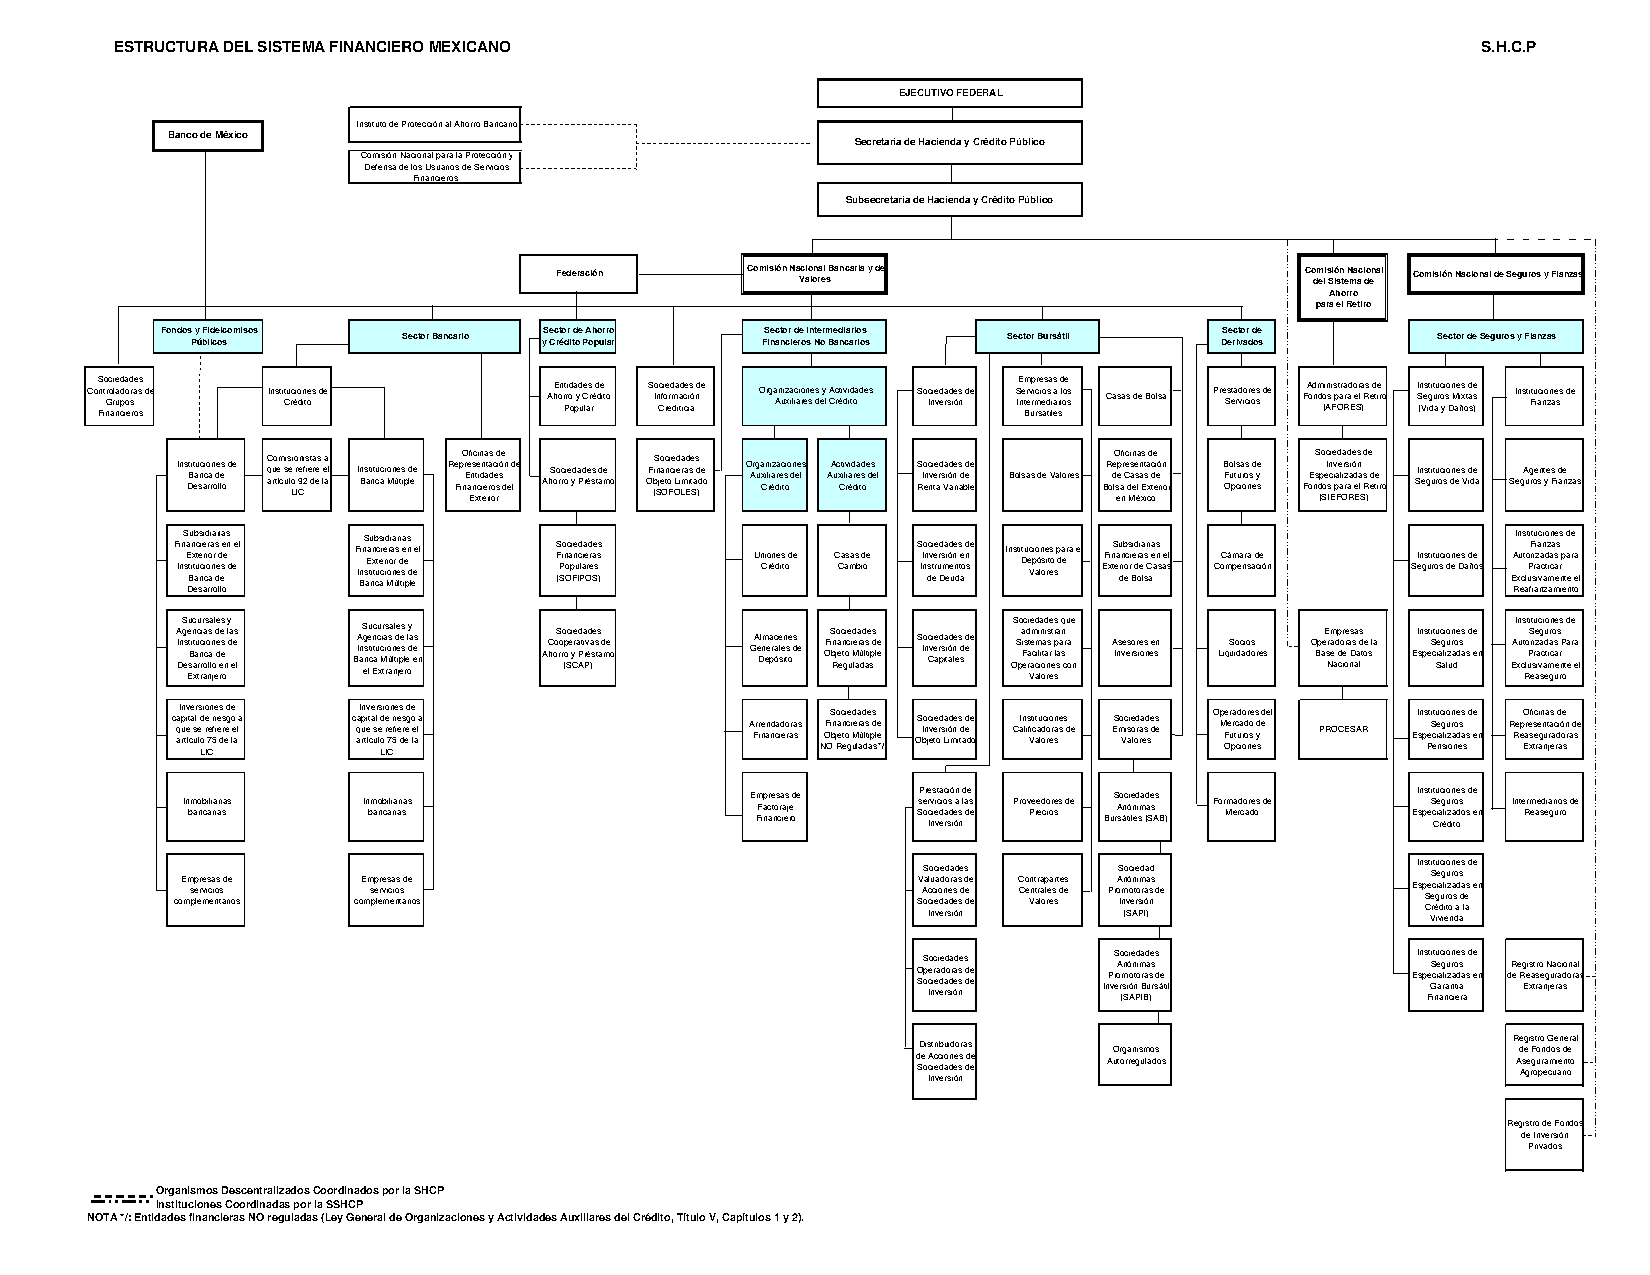
\includegraphics[width=0.5\textwidth]{ea1.pdf}
  \caption{Estructura del sistema financiero}
  \label{ea1}
\end{figure}
Existen otras distinciones importantes de precios en la teoría económica y son:
\begin{itemize}
    \item Precios naturales
    \item Precios de producción
    \item Precio de mercado
\end{itemize}
\subsubsection{Cantidades}
Las cantidades se expresan necesariamente a través de dos atributos: las propiedades intrínsecas de una mercancía y una unidad de medida adecuada a su naturaleza.

Cuando al graficar se obtienen curvas y se intersectan, se obtienen precios de equilibrio
\subsubsection{Valor}
Un valor resulta del producto de un precio por una cantidad es decir:
\begin{equation}
    V = P \cdot Q
\end{equation}
Siendo precisamente ésta la ecuación básica para la comprensión de los fenómenos económicos.

\subsubsection{Utilidad} 
Este concepto corresponde a la valoración estrictamente ordinal y subjetiva de los niveles de satisfacción que logra un consumidor individual con cada canasta de consumo.

Hace posible comparar las posibilidades (canastas) de consumo entre si para evaluar las mejores, las igualmente satisfactorias y las peores a partir de las características específicas de las preferencias del agente económico y eventualmente de sus posibilidades de  financiamiento.

El precio de una mercancía es la cantidad que debe pagarse ahora por la disponibilidad (futura) de una unidad de esta mercancía. El precio de una mercancía puede ser positivo (mercancía escasa), nulo (mercancía libre), o negativo (mercancía nociva).

Obsérvese que no se está haciendo mención a ninguna teoría del dinero y es posible suponer que la economía funciona sin la ayuda de un bien que sirva como medio de cambio. Luego el papel de los precios es el siguiente:
\begin{enumerate}
    \item A cada mercancía se le asocia un número real (su precio)
    \item Cuando un agente económico se compromete a aceptar la entrega de una cierta cantidad, el producto de esta cantidad por el precio de la mercancía es un número real anotado en el debe de su cuenta
\end{enumerate}
\subsubsection{Registro de operaciones del agente A}
\begin{table}[h!]
    \centering
    \begin{tabular}{@{}cc@{}}
    \toprule
    Debe      & Haber \\ \midrule
    $P\dot Q$ &       \\ \bottomrule
    \end{tabular}
    \caption{Cuenta (activo, pasivo, capital, egresos e ingresos)}
    \label{tabe1}
\end{table}
\begin{table}[h!]
    \centering
    \begin{tabular}{@{}cc@{}}
    \toprule
    Debe      & Haber \\ \midrule
              & $P\dot Q$ \\ \bottomrule
    \end{tabular}
    \caption{Registro de operaciones de B}
    \label{tabe2}
\end{table}
El saldo de la cuenta del agente económico es decir el valor neto de todos sus compromisos guía sus decisiones económicas.

% 1,000 si usa terminar se cobra 3\% (NO SE HACE ESO ES ILEGAL) precio del producto o servicio*
% (1000+3\%)= 1,300 COMISIÓN POR USO DE TERMINAL
% SI ME LO PAGAS EN EFECTIVO TE DESCUENTO 

% cosas para comprar facturándolas 

% las que no se hace una contabilidad separada

\begin{example}
    El trabajo humano es considerado como un servicio económico, y su descripción es el de la tarea realizada. 

    Cuando se añade fecha y lugar, se tiene una mercancía buena definida.
\end{example}
Una mercancía es un bien o un servicio completamente especificado física, temporal y especialmente.

Un consumidor es, típicamente, un individuo, puede ser una familia, puede ser incluso un grupo más amplio con un propósito común. Su papel es elegir (y llevar a término) un plan de consumo confeccionado ahora para "todo el futuro", es decir, una especificación de las cantidades de todos sus inputs y todos su outputs.
% Contrato forward
Los inputs de un consumidor cualquiera se representan con números positivos, en tanto que sus outputs con números negativos.

Un productor es un agente económico cuya actividad consiste en elegir (y ejecutar) un plan de producción el cual es confeccionado ahora para la totalidad del futuro y es una especificación de las cantidades de todos sus inputs y todos sus outputs.

Los inputs de una producción pueden comprender por ejemplo, las materias primas, productos semilaborados, terrenos y equipo o sus usos; trabajo delos obreros, ejecutivos en lugares distintos y fechas.

Los outputs son en general más de una mercancía, sólo sean porque la producción involucra varias fechas.

% nan dan yen
Detrás de todos los conceptos y definiciones anteriores se esconden dos ideas claves en la economía:
\begin{enumerate}
    \item Los bienes son escasos y 
    \item La economía debe utilizar los recursos con eficiencia.
\end{enumerate}
Por lo tanto la \textbf{Eficiencia económica}, exige una economía que produzca la combinación más elevada de cantidad y calidad de productos y servicios dada su tecnología y sus escasos recursos. Una economía produce con eficiencia cuando no puede mejorar el bienestar económico de una persona sin afectar negativamente el de otra.

\subsubsection{Microeconomía y macroeconomía}
La forma más sencilla de adquirir una percepción de la amplitud y la profundidad de lo que se estudiará es explorar la forma en la que está organizada la economía:
\begin{itemize}
    \item Microeconomía
    \item Macroeconomía
\end{itemize}
\begin{table}[h!]
    \centering
    \begin{tabular}{@{}ccccc@{}}
    \toprule
    \begin{tabular}[c]{@{}c@{}}División de la\\ economía\end{tabular} &
      Producción &
      Precios &
      Ingresos &
      Empleos \\ \midrule
    Microeconomía &
      \begin{tabular}[c]{@{}c@{}}Producción/producto\\ final de industrias y\\ empresas individuales\end{tabular} &
      \begin{tabular}[c]{@{}c@{}}Precios de bienes y\\ servicios\\ individuales\end{tabular} &
      \begin{tabular}[c]{@{}c@{}}Distribución del\\ ingreso y de la\\ riqueza\end{tabular} &
      \begin{tabular}[c]{@{}c@{}}Empleos por empresas\\ e industrias\\ individuales\end{tabular} \\
    Microeconomía &
      \begin{tabular}[c]{@{}c@{}}Producción/producto\\ nacional\end{tabular} &
      \begin{tabular}[c]{@{}c@{}}Nivel de precios\\ agregado\end{tabular} &
      Ingreso nacional &
      \begin{tabular}[c]{@{}c@{}}Empleo y desempleo\\ en la economía\\ nacional\end{tabular} \\ \bottomrule
    \end{tabular}
    \caption{Ejemplos de aspectos microeconómicos y macroeconómicos}
    \label{tabe3}
\end{table}
\begin{table}[h!]
    \centering
    \begin{tabular}{@{}cc@{}}
    \toprule
    Economía del comportamiento      & Historia del pensamiento económico \\ \midrule
    Sistemas económicos comparativos & Organización industrial            \\
    Econometría                      & Economía internacional             \\
    Desarrollo Económico             & Economía laboral                   \\
    Historia Económica               & Legislación y economía             \\
    Economía ambiental               & Economía política                  \\
    Finanzas                         & Economía urbana y regional         \\
    Economía de la salud             &                                    \\ \bottomrule
    \end{tabular}
    \caption{Los campos de la economía}
    \label{tabe4} 
\end{table}
¿Cómo puede justificarse la existencia de la canasta de consumo? El ser humano demanda bienes en conocimiento de la reparcelación de sustituibilidad y complementariedad que existe de uno cualquiera de los bienes con todos los demás, es decir, ningún bien es independiente de los otros.

Representación matemática de una canasta de consumo: Se piensa en la existencia de n-bienes (de propiedad privada) $Q_1,q_2,q_3$ los seres humanos demandarán canastas de bienes.

Demanda de bienes de un estudiante:
\begin{itemize}
    \item $Q_1=$ gasolina, internet, agua, computadora, telefonía, libretas, bolígrafos
    \item $q_2=$ Leche, servicios sanitarios, cama, pan
\end{itemize}
Demanda de bienes de
\begin{itemize}
    \item $q_1=$ Agua, internet, telefonía, vestido, tortillas, computadora, cobijas, servicios, sanitarios, electricidad, gas
    \item $q_2=$ Huevos, harina, café, zapatos, pan.
\end{itemize}
\section{Microeconomía}
Cuando un consumidor demanda algo, significa que:
\begin{itemize}
    \item Lo desea
    \item Tiene la capacidad de adquirirlo
    \item Tiene planes para comprarlo
\end{itemize}
La cantidad demandada de un bien o servicios es el monto que los consumidores planean comprar durante un periodo determinado, a un precio específico\footnote{La cantidad demandada no es necesariamente la cantidad adquirida en la realidad}

De acuerdo con la definición de cantidad demandada, ésta se mide en términos de monto por unidad de tiempo. Muchos son los factores que influyen en los planes de compra y entre ellos es el precio.

Para analizar dicha relación, se mantendrán sin cambio los demás factores que influyen en los planes de compra.

¿Cómo, si el recto de los factores permanece sin cambio, se modifica la cantidad demandada de un bien conforme el precio cambia?

Ley de la demanada: Si los demás factores, cuanto más alto es el precio de un bien, menor es la cantidad demandada del mismo; y a menor precio de un bien, mayor es la cantidad demandada.
% visa mastercad
% rooming
\subsection{Teoría del consumidor}
\begin{example}
\label{exae1}
    Construir una curva de demanda para agua embotellada en presentación de () de la marca: (). Consulte los precios en cinco páginas de internet de tiendas de autoservicio así como en el mercado local. Considere una restricción presupuestal semanal de () pesos semanales.
    \begin{table}[h!]
        \centering
        \begin{tabular}{@{}ccc@{}}
        \toprule
        Establecimiento & Precio Unitario & Cantidad \\ \midrule
        Walmart         & 12              & 26.67    \\
        Soriana         & 15.7            & 20.38    \\
        Farmacia G.    & 15.5            & 20.65    \\
        La meche           & 15              & 21.33    \\ \bottomrule
        \end{tabular}
        \caption{Restricción presupuestaria de \$320}
        \label{tabe5}
    \end{table}
    Graficándola, queda:
    \begin{figure}[h!]
    \centering
      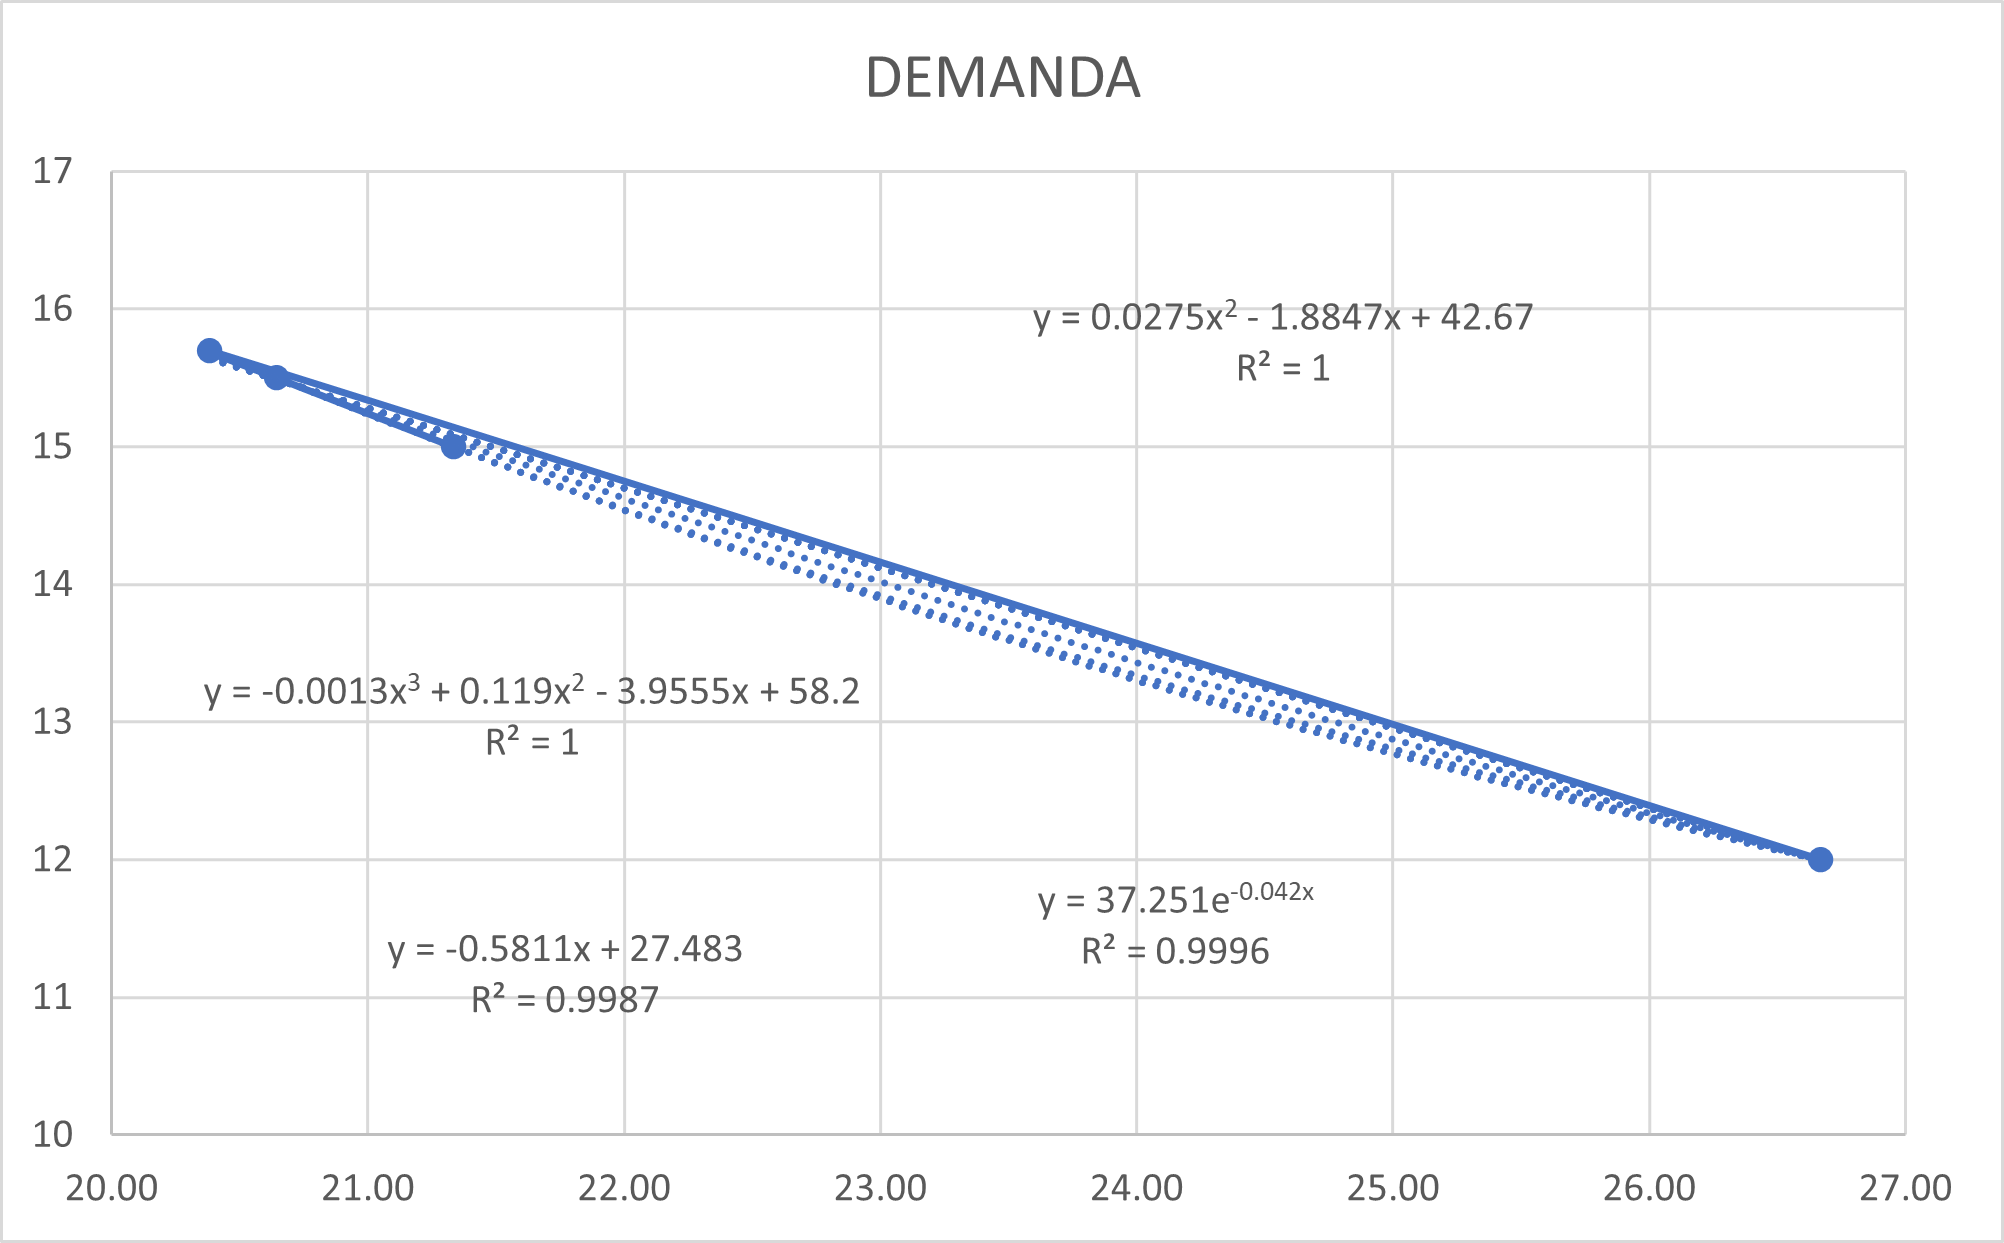
\includegraphics[width=0.5\textwidth]{ea2.png}
      \caption{Curva de la demanda}
      \label{ea2}
    \end{figure}
\end{example}
Dada la naturaleza de los precios, es posible observar que la curva de la demanda no pasa por todos los puntos, sin embargo, crea una tendencia, en este caso se realizó una interpolación de tipo exponencial y es la que determina la citada tendencia.

En la curva interpolada de demanda, se deben identificar dos tipos de movimiento
\begin{enumerate}
    \item Cambio en la cantidad demandada: movimiento a lo largo de la misma
    \item Cambio en la tendencia: Ocurre cuando cualquiera de los supuestos ceteris paribus baría y en este caso hay un desplazamiento de toda la curva.
\end{enumerate}
Si en la canasta de consumo no se incluye un bien (ya sea un bien de lujo), supóngase que aumenta la beca y que ahora tendría una asignación de \$480 semanales para gastar en agua bajo esta nueva condición, la curva quedará como:
\begin{figure}[h!]
\centering
  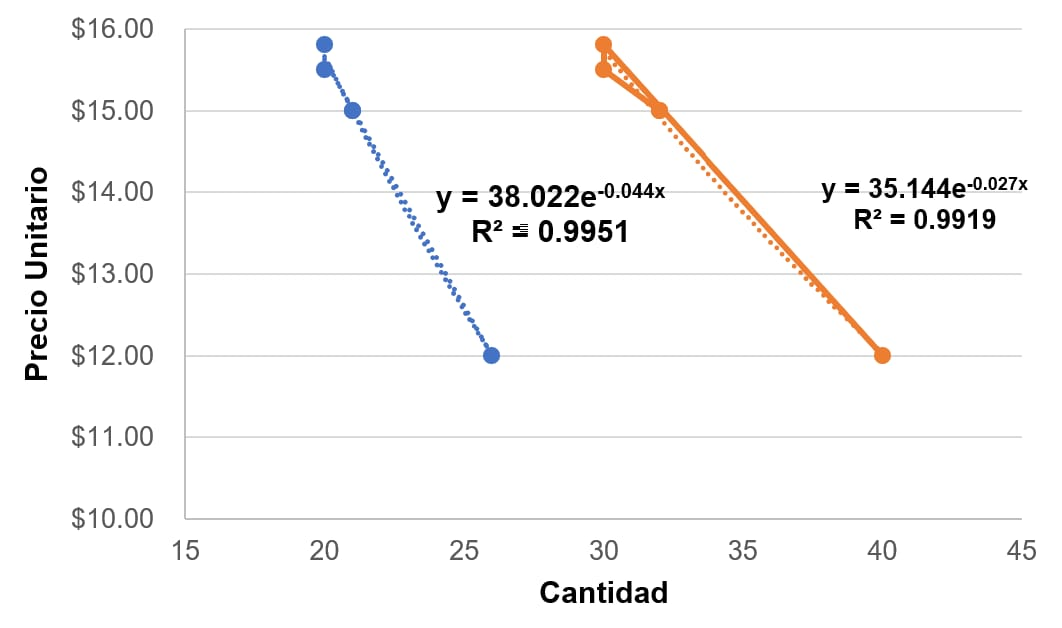
\includegraphics[width=0.5\textwidth]{ea3.jpg}
  \caption{Curva de la demanda con el aumento de ingresos $f(p,q)= 480$}
  \label{ea3}
\end{figure}
Estas curvas son las curvas de la figura \ref{ea3} de nivel de una función que está en el espacio $\mathbb{R}^3$

Para el ejemplo \ref{exae1}, como pudo observarse, un aumento en el ingreso semanal provocó el desplazamiento de la curva de demanda hacia la derecha. Sin embargo, no es el único factor, existen seis posibles:
\begin{itemize}
    \item Precios de bienes relacionados
    \item Precios esperados en el futuro
    \item Ingreso
    \item Ingreso esperado en el futuro y crédito
    \item Población
    \item Preferencias.
\end{itemize}
\subsubsection{Precios de bienes relacionados} 
La cantidad de botellas de agua que los consumidores planean comprar depende en parte de los precios de los sustitutos de este artículo: \textbf{Un sustituto es un bien que puede utilizarse en lugar de otro.}

\begin{example}
    Un viaje en autobús es un sustituto de un viaje en metro; una hamburguesa es un sustituto de un sándwich y una bebida hidratante o un suero es un sustituto de una botella de agua. SI el precio de un sustituto de una botella de agua, por ejemplo el Gatorade, disminuye, la gente comprará más unidades de ese sustituto y menos botellas de agua y con ello disminuye la demanda de botellas de agua.
\end{example}

\subsubsection{Precios de bienes relacionados}

La cantidad de botellas de agua que la genet planea comprar también depende de los precios de sus complementos: Un complemente es un bien que se utiliza en conjunto con otro.

Por ejemplo la hamburguesas y las papas fritas son complementos entre sí, lo mismo que las botellas de agua y el ejercicio. Si el precio de una hora en el gimnasio baja, la gente comprará más tiempo en el gimnasio y más botellas de agua.

\subsubsection{Precios esperados en el futuro} 
Si se espera que el precio de un bien aumente en el futuro y dicho bien puede almacenarse, el costo de oportunidad de obtener el bien para su uso futuro es menor hoy de lo que será cuando el precio haya aumentado. Por esta razón, la gente reprograma sus compras; es decir, hace una sustitución temporal comprando más del bien ahora (y menos después), antes de que su precio suba, lo que provoca que la demanda actual del bien aumente.

De manera similar, si se espera una disminución futura en el precio de un bien, el costo de oportunidad de comprar dicho bien ahora es más alto que en el futuro. Una vez más, la gente reprograma sus compras. compra menos del bien ahora, antes de que su precio baje, lo cual provoca que la demanda del bien disminuya hoy y aumente en el futuro.

\subsubsection{Ingreso}
El ingreso de los consumidores también influye en la demanda. Cuando el ingreso aumenta, los consumidores compran más de casi todos los bienes; Cuando éste disminuyen los consumidores compran menos de casi cualquier bien. Aunque un aumento en el ingreso conlleva a un incremento en la demanda de la mayoría de los bienes, este incremento en la demanda no se extiende a todos los bienes.

Un bien normal es aquel cuya demanda se incrementa conforme el ingreso aumenta; un bien inferior es aquel cuya demanda baja conforme el ingreso aumenta.
\begin{example}
    Cuando los ingresos suben, la demanda de viajes aéreos (un bien normal) aumenta, mientras la demanda de viajes largos en autobús (un bien inferior) disminuye
\end{example}
\subsubsection{Ingreso esperado en el futuro y crédito}
    Cuando se espera que el ingreso aumente, en el futuro o cuando el crédito es fácil de obtener la demanda podría aumentar en el presente.
\begin{example}
    Un trabajador recibe la noticia de que recibirá en el transcursos del año el reparto de utilidades y el aguinaldo, por lo que decide comprar un automóvil nueva ahora
\end{example}

\subsubsection{Población}
La demanda también depende del tamaño y la distribución por edades de la población. Cuanto más grande sea la población, mayor será la demanda de todos los bienes y servicios; cuanto menos numerosa sea la población, menor será la demanda de todos los bienes y servicios.

Asimismo, cuanto más grande sea la proporción de la población de un grupo de edad determinado, mayor será la demanda de bienes y servicios utilizados por ese grupo de edad. 
\subsubsection{Preferencias}
La demanda también depende de las preferencias. Las preferencias determinan el valor que la gente le da a cada bien y servicio. Las preferencias dependen de cosas como el lima, la información y la moda.

\begin{example}
    Un mayor interés por la salud y la condición física ha cambiado las preferencias a favor de los suplementos alimenticios, por lo que la demanda de este tupo de bienes ha aumentado.
\end{example}
\subsection{Teoría del productor}
Si una empresa ofrece un bien o servicio, significa que dicha empresa:
\begin{enumerate}
    \item Cuenta con los recursos y la tecnología para producirlo
    \item Puede obtener un beneficio al productor
    \item Ha elaborado un plan definido para producirlo y venderlo
\end{enumerate}
Una oferta implica más que sólo contar con los recursos y la tecnología para producir algo. Los recursos y la tecnología constituyen los límites de lo posible y es posible producir muchas cosas útiles, pero éstas no serán fabricadas a menos que hacerlo resulte lucrativo.

La cantidad ofrecida de un bien o servicio es la suma que los productores planean vender durante un periodo dado a un precio específico y la cantidad ofrecida no necesariamente es la misma cantidad que se venderá en realidad.

Al igual que la cantidad demandada, la cantidad ofrecida se mide en un monto por unidad de tiempo.

Son muchos los factores que influyen en los planes de venta y como antes, uno de ellos es el precio.

De nuevo, como se hizo antes al analizar la demanda, para aislar esta relación, se mantendrá constante todos los demás factores que influyen en los planes de venta y entonces tiene lugar la pregunta ¿Cómo cambia la cantidad ofrecida de un bien conforme su precio cambia, cuando toros factores permanecen sin cambios?

La respuesta a la pregunta, da la ley de la oferta

\begin{definition}[Ley de la oferta]
    Si los demás factores permanecen constantes, cuanto más alto sea el precio de un bien, mayor será la cantidad ofrecida de éste, y cuanto más bajo sea el precio de un bien, menor será la cantidad ofrecida del mismo.
\end{definition}
El término oferta se refiere a la relación completa entre el precio de un bien y la cantidad ofrecida del mismo y se representa como un punto sobre la curva de oferta.

La oferta se ilustra mediante la curva de oferta y el plan de oferta.

¿Por qué un precio más alto aumenta la cantidad ofrecida?

Porque el costo marginal aumenta.

Conforme la cantidad producida de cualquier buen se incrementa, el costo marginal de producirlo también lo hace.

No vale la pena producir un bien si el pago recibido por él no cubre por lo menos el costo marginal de su producción. Por ello, cuando el precio de un bien aumenta pero el restos de los factores permanece igual, los productores están dispuestos a incurrir en un costo marginal más alto y aumentar la producción. Este precio más alto ocasiona un aumento en la cantidad ofrecida.

\begin{example}
    Considérese un productor que radica en el estado de Colima que tiene la disyuntiva de elegir entre dos posibles cultivos (Plátano y papaya, sin mencionar detalles de variedades) con buena rentabilidad en ambos. 

    El productor cuenta con un terreno tal que puede tener 20 hectáreas efectivas para cultivar.
    \begin{enumerate}
        \item Construya la FPP para el productor (Consulte los datos necesarios de la página web del FIRA)
        \item Construya la curva de oferta para el productor
    \end{enumerate}


    \textit{ Sol. }


    \begin{table}[h!]
        \centering
        \begin{tabular}{@{}ccccc@{}}
        \toprule
        Cultivos &
          \begin{tabular}[c]{@{}c@{}}Rendimiento\\ t/ha\end{tabular} &
          \begin{tabular}[c]{@{}c@{}}Precio de venta\\ t/ha\end{tabular} &
          \begin{tabular}[c]{@{}c@{}}Costos de\\ Producción\end{tabular} &
          \begin{tabular}[c]{@{}c@{}}Utilidad del\\ ciclo\end{tabular} \\ \midrule
        Plátano &
          65 &
          \$6,000 &
          \$2024 &
          \$5,168,800 \\
        Papaya &
          47 &
          \$ 5,500 &
          \$ 3,445 &
          \$1,931,700 \\ \bottomrule
        \end{tabular}
        \caption{Elaboración propia con datos de la página de Fira}
        \label{tabe6}
        \end{table}
\end{example}
\begin{definition}[Frontera de posibilidades de productor]
    Representa las cantidades máximas de un par de bienes o servicios que pueden producirse con los recursos dados en una economía en el supuesto de que todos ellos se utilizan en plenitud.
\end{definition}

\begin{definition}[Costo de oportunidad]
    Las decisiones tienen costos de oportunidad porque elegir una cosa en un mundo de escasez significa renunciar a otra. El costo de oportunidad es el valor del bien o servicio más valioso al que se renuncia.
\end{definition}
La curva de oferta indica la relación entre la cantidad ofrecida y el precio si todos los demás factores permanecen sin cambio.

Este tipo de curva describe una pendiente positiva: Conforme el precio de un bien aumenta, también lo hace la cantidad ofrecida.

Así mismo, la curva de oferta puede interpretarse como una curva de precio mínimo de oferta, ya que indica el precio más bajo al que alguien está dispuesto a vender y este precio más bajo es el costo marginal.
\begin{definition}[Curva de Oferta]
    Si la cantidad producida es pequeña, el precio más bajo al que alguien estará dispuesto a vender una unidad adicional es relativamente bajo. Pero a medida que la cantidad producida aumenta, el costo marginal de cada unidad adicional aumenta el precio más bajo al que alguien estará dispuesto a vender también aumenta a lo largo de la curva de oferta.
\end{definition}
Cuando cualquiera de los factores que influyen en los planes de venta distinto al precio del bien cambia, se genera un cambio en la oferta. Y básicamente puede atribuirse a seis factores los cuales pueden considerarse como principales:
\begin{itemize}
    \item Precios de los recursos productivos (insumos): Son bienes que satisfacen una misma necesidad o una de muy similar y, por lo tanto, pueden ser reemplazados por otro bien según los factores que decanten la decisión del comprador (como el precio).
    \item Precios de los bienes relacionados producidos
    \item Precios esperados en el futuro: Aplicado en contrato forward
    \item Número de proveedores: Si son escasos, los precios son caros
    \item Tecnología
    \item Estado de la naturaleza
\end{itemize}
\section{Equilibrio de mercado}
La oferta de un bien o servicio:

\textbf{Disminuye si}: El precio de uno de los recursos usados en la producción sube, el precio de un sustituto en la producción sube; El precio de un complemento en la producción baja; Se espera que el precio del bien o servicio aumente en el futuro; El número de proveedores del bien o servicio disminuye; Ocurre un cambio tecnológico que disminuye la producción del bien o servicio; Un fenómeno natural provoca una disminución en la producción.

\textbf{Aumenta si}: El precio de uno de los recursos utilizados en la producción del bien o servicio baja; EL precio de un bien o servicio sustituto en la producción baja; EL precio de un complemento de un bien o servicio sube; Se espera que el precio de un bien o servicio baje en el futuro; El número de proveedores del bien o servicio aumente; Ocurre un cambio tecnológico que disminuye la producción del bien o servicio y Un fenómeno natural provoca un aumento en la producción.

Cuando se ponen en contacto a consumidores y productores con sus respectivos planes de consumo y producción, esto es, con sus respectivas curvas de oferta y demanda en un mercado particular, es posible analizar como se lleva a cabo la coordinación de ambos agentes.

En los mercados, el equilibrio ocurre cuando el precio hace que los planes de compradores y vendedores concuerden entre si.
\begin{definition}[Precio de equilibrio]
    Es el precio al que la cantidad demandada es igual a la cantidad ofrecida.
\end{definition} 
La cantidad de equilibrio es la cantidad comprada y vendida al precio de equilibrio, los mercados tienden al equilibrio debido a:
\begin{itemize}
    \item El precio regula los planes de compra y venta
    \item El precio se ajusta cuando los planes no concuerdan.
\end{itemize}
Para comprender por qué los mercados tienden a equilibrarse, supóngase que el precio fuera inicialmente superior al que los equilibra, por ejemplo $P_1$.

Los productores tratarán de producir y vender más de lo que los consumidores están dispuestos a comprar. Habrá un excedente, es decir, una situación en la que la cantidad ofrecida es superior a la cantidad demandada. Para venderlo o para impedir, al menos, que siguiera creciendo, luego los productores comenzarán a bajar los precios. Finalmente, al descender el precio, la cantidad demandada aumentará y la cantidad ofrecida disminuiría hasta que se alcance el precio de equilibrio $P_0$.

Ahora considérese el caso si el precio fuera inicialmente inferior a $P_0$ por ejemplo, $P_2$ ocurriría lo contario.

Habría escasez, una situación en la que la cantidad demandada es superior a la ofrecida, por lo que los consumidores no podrían comprar todo lo que les gustaría. Eso presionaría al alza sobre el precio, la que los consumidores tratarían de presionar más que los demás por las existencias y los productores reaccionarían elevando el precio e incrementando la producción. Una vez más, el precio acabaría alcanzando el nivel $P_0$.
\begin{figure}[h!]
\centering
  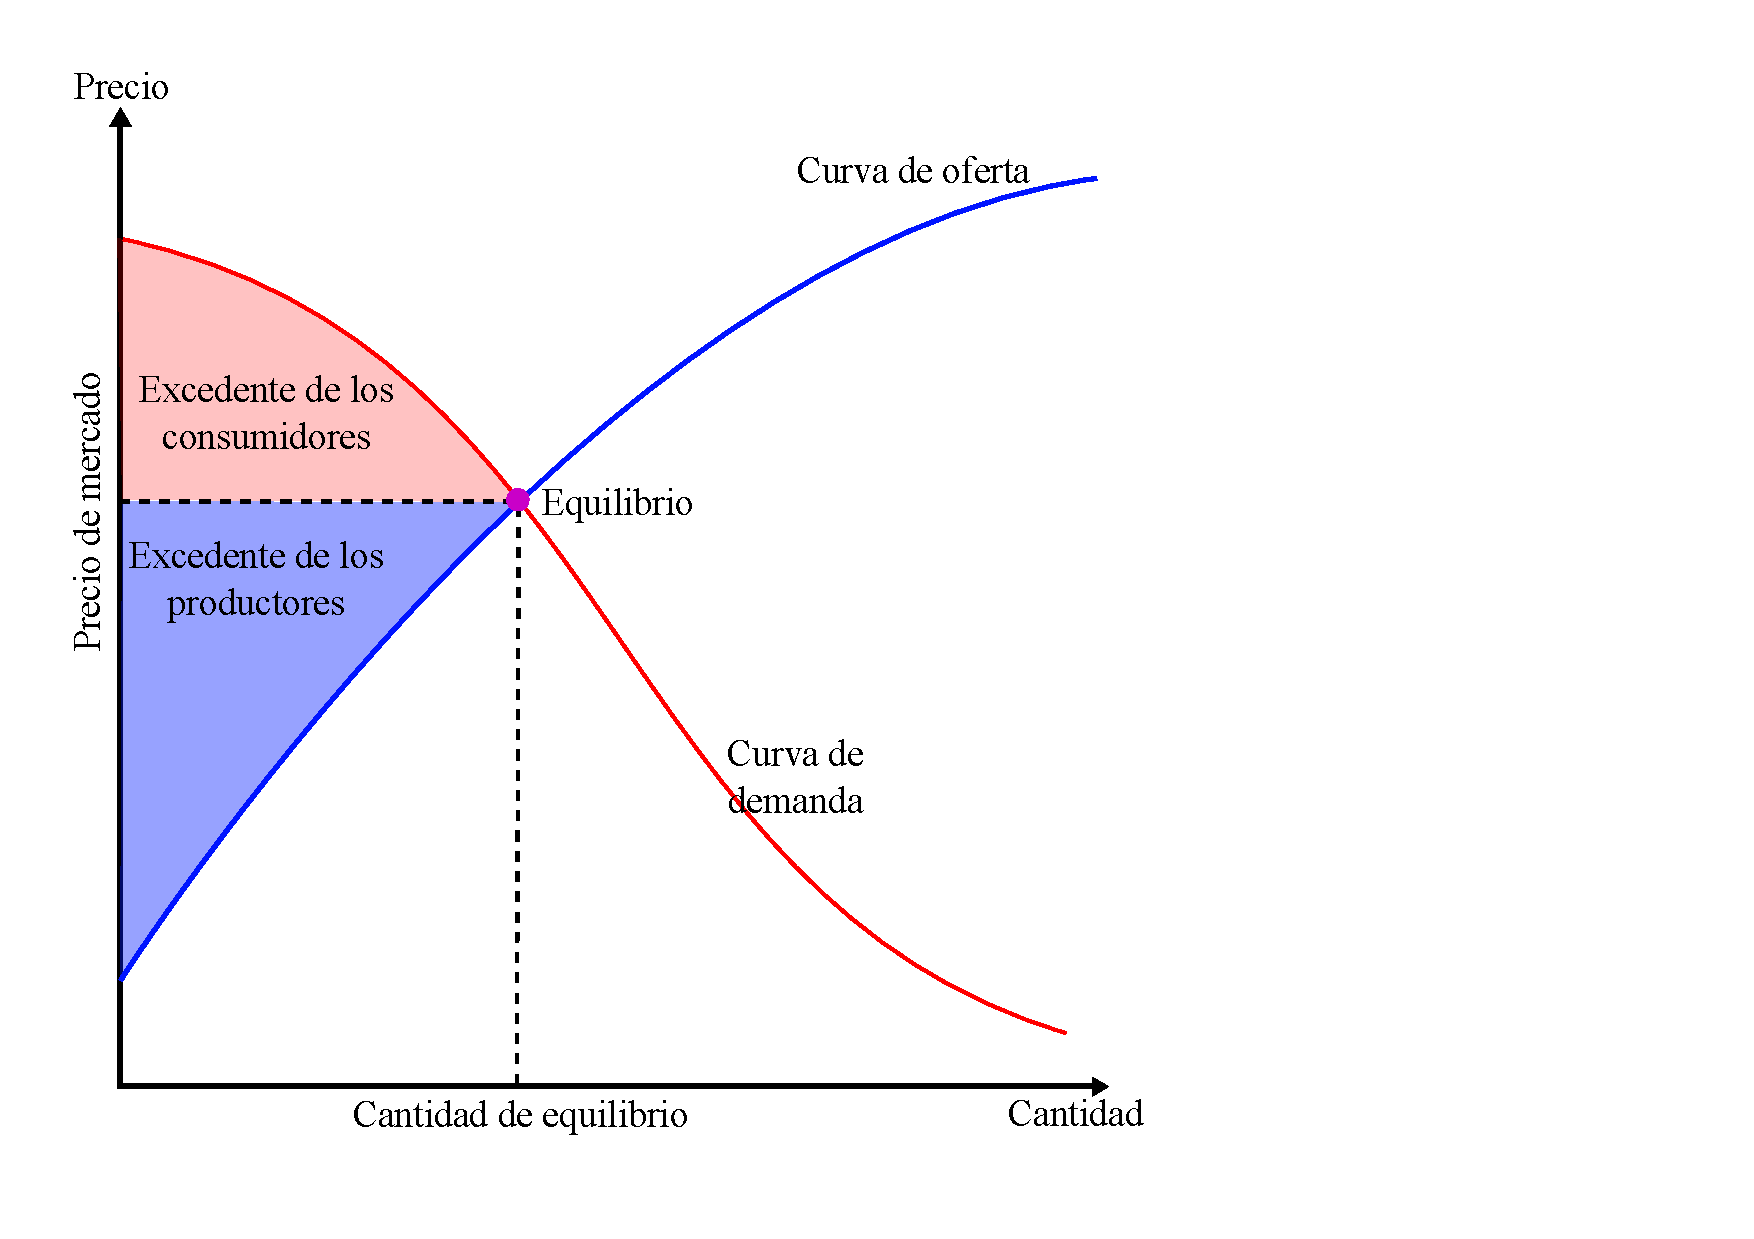
\includegraphics[width=0.5\textwidth]{ea4.pdf}
  \caption{Excedente de los consumidores y los productores en el punto de equilibrio para las curvas de oferta y demanda}
  \label{ea4}
\end{figure}
\section{Producción y Costos}
Las personas responsables de las operaciones de las empresas toman muchas decisiones, todas las cuales responden a un objetivo primordial: Maximizar las utilidades económicas.

Así, una de las decisiones más importantes que tiene una empresa es decidir a qué industria ha de ingresar. Y realizado esto, el siguiente paso es saber sobre la cantidad a producir y el precio a cobrar, el cual depende del tipo de mercado donde operará la empresa.

Los mercados pueden ser de:
\begin{itemize}
    \item Competencia perfecta
    \item Competencia Monopolística
    \item Oligopolio y Monopolio
\end{itemize}
En cualquiera de los casos, cada mercado presenta sus propios problemas específicos.

Por lo tanto las acciones que una empresa puede llevar a cabo para influir en la relación entre la producción y los costos dependen de qué tan rápido se quiera actuar.

Para analizar la relación entre la decisión de producción de una empresa y sus costos, se debe distinguir entre dos marcos de tiempo de las decisiones: Corto y largo plazo.

A corto plazo es un marco de tiempo en el cual las cantidades de algunos recursos son fijas

Para la mayoría de las empresas, el capital, la tierra y las habilidades empresariales son recursos fijos, mientras que el trabajo es el recurso variable.

Al conjunto de recursos fijos de la empresa se le denomina planta: por lo tanto, la planta de una empresa es fija en el corto plazo.

\begin{example}
Una planta fija está constituida por el edificio donde reside una fábrica y por su maquinaria.

Si fuera el caso de una planta de generación de energía eléctrica, la planta fija está constituida por sus edificios, generadores, computadores y sistemas de control (entre otros).

Para aumentar la producción en le corto plazo, una empresa debe incrementar la cantidad de un recurso variable por lo general el trabajo.
\end{example}
Por lo tanto, para generar mayor producción, en el caso de la planta de generación de energía debe contratar más trabajadores y operar sus generadores durante más horas por día.\footnote{Las decisiones a corto plazo pueden revertirse fácilmente.}

La empresa puede aumentar o disminuir su producción en el corto plazo, aumentado o disminuyendo la cantidad de trabajadores que contrata.

El largo plazo es un marco temporal en el que las cantidades de todos los factores de producción pueden variar. Es decir, el largo plazo es un periodo en el que la planta de la empresa puede cambiar para aumentar la producción en el largo plazo, la empresa está en posibilidad de elegir si cambiar su planta o la cantidad de trabajo que contrata, o decidir si debe instalar alguna máquinas adicionales, utilizar un nuevo tipo de máquina, reorganizar a sus gerentes o contratar más trabajadores.\footnote{Las decisiones a largo plazo no se revierten con facilidad}

Una vez que se ha tomado una decisión con respecto a la planta, por lo general la empresa tiene que mantenerse firme en ella por cierto tiempo.

Para enfatizar esto, al gasto hecho en el pasado en una planta sin valor de reventa lo llamamos costo perdido.

Los costos perdidos son irrelevantes para las decisiones actuales de la empresa. Los únicos costos que influyen en sus decisiones son el costo a corto plazo de cambiar sus insumos de trabajo y el costo a largo plazo de cambiar su planta.

Para aumentar la producción a corto plazo, a empresa debe incrementar la cantidad de trabajo que emplea, la relación entre la producción y la cantidad de trabajo empleado se describe mediante tres conceptos relacionados:
\begin{enumerate}
    \item Producción total
    \item Producto marginal
    \item Producto medio
\end{enumerate}
Estos conceptos sobre el producto pueden ilustrarse ya sea a través de planes de producto o mediante curvas de producto.

\subsubsection{Planes de producto}
\begin{definition}[Producto total]
    Es la producción máxima que se puede generar con una cantidad de trabajo determinada
\end{definition}

\begin{definition}[Producto marginal del trabajo]
    Es el aumento del producto total como resultado de aumentar en una unidad la cantidad de trabajo empleado cuando todos los demás insumos permanecen constantes
\end{definition}

\begin{definition}[Producto medio del trabajo]
    es igual al producto total dividido entre la cantidad de trabajo empleado.
\end{definition}





































